
\section{Size Limits (lower bounds) for Effective Transfer Learning}
\label{sec:sizelimit}

In this section, we investigate the lower bounds of the effective sizes of source and target datasets for HDP models to address RQ2.

{\bf RQ2: What are the  lower  bounds  of  the  size  of source and target  datasets  for  effective HDP?}

Since HDP compares the distributions of source metrics to those of target metrics, it is important to seek the empirical evidence for the effective sizes of source and target datasets to match source and target metrics. We first present the results of the empirical study for RQ2 in Section~\ref{sec:sizelimit} and validate the generality of its results in Section~\ref{sect:xplain}.

Like prior work \cite{Nam13,
  Ma12, Rahman12, Ryu14,
  Zhang14}, the basic HDP method we
proposed above uses {\em all} the instances in potential source and target data to
perform KS-test to select the best matched metrics and then build
defect prediction learners.
Collecting {\em all} that data from source and target projects need much more work and also
for the target project, it requires waiting for it to finish before
transferring its learned lessons. This begs the question ``how early can we transfer?''.
That is, how {\em few} data from source and target projects do we need before transfer can be effective? In this section, we conduct an empirical study to answer these questions related to RQ2.

To investigate the size limits for effective transfer learning in the setting of CPDP across datasets with heterogeneous metric sets, we focus on the HDP approach. There are other approaches such as CPDP-IFS~\cite{He14} and CCA+~\cite{Jing15}. In Section~\ref{sec:Result}, we observed that HDP outperforms CPDP-IFS. In addition, CCA+ was evaluated in somewhat different context, i.e., cross-company defect prediction and with 14 projects which are far less than 28 projects used in our experiments for HDP. In addition, the implementation of CCA+ is not publicly available yet and more complex than HDP. For this reason, we conducted our empirical study for RQ2 based on HDP.

\begin{figure}[t]
	\centering
% 	\vspace{0.5mm}
	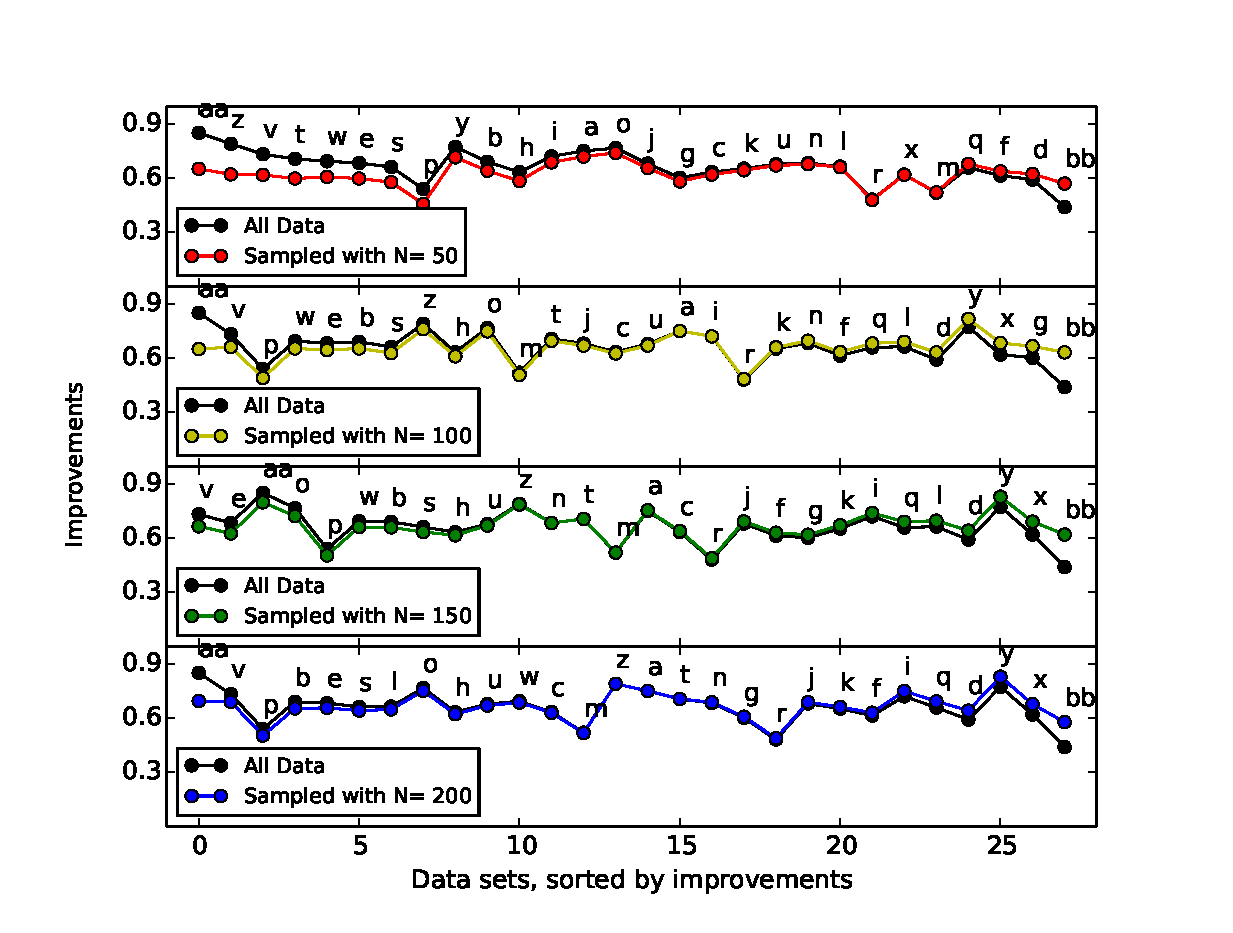
\includegraphics[width=\linewidth]{Figures/raleigh/sample_random.eps}
	\caption{Improvements of using sampled data over all data with sampled size N = \{50, 100, 150, 200\}. We label the data in table \ref{tab:datasets} from a to z, and the last two datasets ar5 and ar6 as A and B.}
	\label{fig:small_data}
\end{figure}


\subsection{200 Random Samples are Enough}

Recall from the above,
HDP uses  datasets  in a two step process.
To test the impact of having access to {\em less} data,
we  add an instance sampling process before performing metric matching:
instead of using all the instances from
candidate source and target datasets, those datasets will
be randomly sampled to generate smaller datasets of
size $N \in \{50, 100, 150, 200\}$. If
the number of instances in the original dataset is
smaller than $N$, all those instances will be
included. With those sampled data, we perform metric matching to build a learner
and finally predict labels of all original data in the target project.

The results for this HDP-with-limited-data experiment is shown in \fig{small_data}
(we display median AUC results from 20 repeats, using  Logistic Regression
as the default learner). 
% \lin{It's unclear to me. So metric matching on the 50, 100, etc.? What is third initial sampling? Add a backward reference to it? One caveat: I focused on reading the abstract, Section 3, 7, and 8, and I only skimmed over the rest of the paper, so maybe I missed it. But in general it is still good to add a backward reference.}\wei{I didn't get the question, "what is third initial sampling?", which third?}
% Since {\it Apahce commons math} library takes quite long time to conduct KS-test as mentioned, we replace it with Scipy, a python package, to speed up our experiment. \footnote{As shown in the table, the difference between those two KS-test results is acceptable}.
In that figure:
\squishlist
\item
  The {\em black} line show the results using {\em all} data;
\item
  The {\em colourful} lines show results of transferring from {\em some} small $N$ number of samples (instead of {\em all})
  in the source and target datasets during metric matching and learner building;
\item
  The letters show the unique ID of each dataset.
\squishend
The datasets are ordered left to right by the difference to the black line (where we transfer using {\em
  all} the source data):
\squishlist
\item
  On the left, the black line is
  {\em above} the red line; i.e. for those datasets, we do {\em better} using
  {\em all} data than using {\em some}.
  \item
On the right, the black line is {\em below} the red
line; i.e. for those datasets, we do {\em worse}
using {\em all} data than using {\em some}.
\squishend

Note that the gap between the red and black line
shrinks as we use more data and after $N=100$, the
net gap space is almost zero.  When $N=200$, $27/28$
tests are within 0.05 difference in terms of AUC and
$17/28$ tests show smaller datasets have equivalent
or even better performance. Here, we recommend that
sample size $N=200$ could be good enough for this
HDP framework to obtain a good predictor.



\begin{figure}[t]
	\centering
% 	\vspace{0.5mm}
	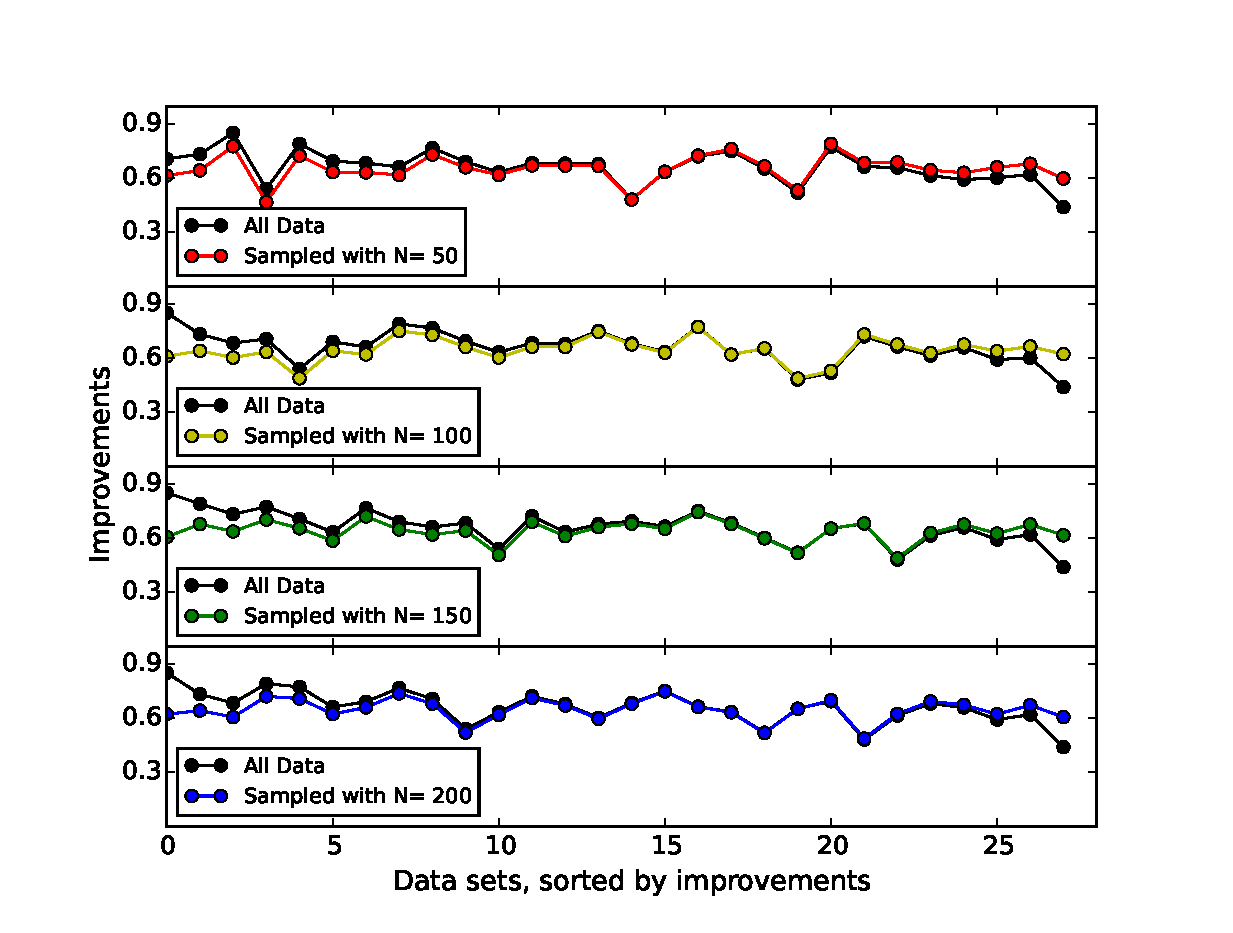
\includegraphics[width=\linewidth]{Figures/raleigh/sample_epv.eps}
	\caption{Improvements of using sampled data N  = \{50, 100, 150, 200\} with EPV constraints. We label the data in table \ref{tab:datasets} from a to z, and the last two datasets ar5 and ar6 as A and B.}
	\label{fig:small_epv}
\end{figure}


\subsection{20 Defective Examples  are Enough}


The results of the last section are very encouraging---a small number of source
and target examples are enough for effective transfer learning. Naturally,
we were suspicious of this result (since it was ``almost too good to be true'').
Accordingly, we explored the literature and found:
\squishlist
    \item Evidence that this ``a few examples are enough'' has been seen in other domains~\cite{peduzzi1996simulation}; 
    \item Methods to reduce the cost of sampling this dataset, even further. 
\squishend
Working in the domain cardiology,
  Peduzzi et al.~\cite{peduzzi1996simulation}
  report 10 ``events'' per variable (EPV) are enough to maximize the predictive performance
  of  Logistic Regression (the learner used in this study). Translated into our terminology,
  that study would predict that  10 defective data per independent variable should
  suffice for effective learning. Of course, learners require defective and {\em non-defective}
  examples so to $M$ defective examples, we add $(N-M)$ non-defective examples more.

  To apply the method of Peduzzi et al., we first instrumented HDP to determine how many
  independent variables were picked during {\em metric  selection}. In practice, that number
  was very small: usually just 2. Hence, applying  Peduzzi et al.'s rule (EPV=10), we picked $2\times 10=20$ %\lin{why *10?}\wei{EPV=10, mentioned in the last paragraph. }
  randomly selected defective data, then randomly added $(N-M)$ non-defective data for
  $N\in \{50,100,150,250\}$ for the source data. For the target dataset, since we do not
  know the data labels, we simply sampled $N$ for target data in metric matching.

  (Aside: note that this is different to the above experiment since, before, the more $N$ examples
  we selected, the more {\em defective} instances we would use. Now, in this experiment, we will also
  use a fixed $M=20$ number of defects.).

  The results are shown in \fig{small_epv}. Like before:
\squishlist
  \item These are median AUC results from 20 repeats;
\item
  The {\em black/colourful} lines show the results using {\em all/some} of  data from
  the source and target datasets during metric matching and learner building, respectively
  (but now, the {\em some} never contains more than $M=20$ defective instances);
\item
  The datasets are ordered left to right according
  the performance difference between using
   {\em all} or {\em some} of the data;
   \item
     On the left/right ,  we do {\em better/worse} using
  {\em all} data than using {\em some}.
\squishend
  We observe that between $N=50$ and $N=200$, the performance delta
  does not change by much. Also, if we compare $N=200$ between \fig{small_data}
  and \fig{small_epv}, there is no large disadvantage of using just
  $M=20$ defective instances.

  Note that such a very small sample would be quick to collect: after writing (say) a few
  hundred classes, inspect enough to find 20 defective ones---at which point that data is a candidate
  for transfer learning.
